\documentclass[11pt]{report}
\usepackage[utf8]{inputenc}
\usepackage[margin=2.0cm]{geometry}
\usepackage{fancyhdr}
\usepackage{xcolor}
\usepackage{minted}
\usepackage{graphicx}
\usepackage[parfill]{parskip}
\usepackage{tabularx,colortbl}

\title{Digital Engineering\\Lab 4}
\author{Y3890959\\Y3878784}
\date{14th February 2023}

\pagestyle{fancy}
\fancyhead{}
\setlength{\headheight}{14pt}
\fancyhead[L]{Lab 4}
\fancyhead[R]{Y3890959, Y3878784}
\fancyfoot{}
\fancyfoot[L]{Digital Engineering}
\fancyfoot[R]{\thepage}

\makeatletter
\let\ps@plain\ps@fancy 
\makeatother

\setminted {
    fontsize=\footnotesize,
    frame=single,
}

\begin{document}

\maketitle

\chapter*{Task A: Test Pattern Generation}

\section*{3.1.1 Gate Level Fault Collapsing}
Key: The inputs are X and Y. The output is Z. The outputs that don't match the desired have been highlighted yellow to show that the fault can be detected.

\subsection*{AND Gate}
\begin{tabular}{ |c|c|c|c|c|c|c|c| }
\hline
INPUT XY & DESIRED Z & Xs-a-0 & Xs-a-1 & Ys-a-0 & Ys-a-1 & Zs-a-0 & Zs-a-1
\\ 
\hline
\hline
00 & 0 & 0 & 0 & 0 & 0 & 0 & \cellcolor{yellow!50}1
\\  
\hline
01 & 0 & 0 & \cellcolor{yellow!50}1 & 0 & 0 & 0 & \cellcolor{yellow!50}1
\\
\hline
10 & 0 & 0 & 0 & 0 & \cellcolor{yellow!50}1 & 0 & \cellcolor{yellow!50}1
\\
\hline
11 & 1 & \cellcolor{yellow!50}0 & 1 & \cellcolor{yellow!50}0 & 1 & \cellcolor{yellow!50}0 & 1
\\
\hline
\end{tabular}

Looking at the last row in the table above, we've for one test vector `11' being able to test 3 faults (Xs-a-0, Ys-a-0, and Zs-a-0) these faults are equivalent.
Looking at the middle two rows with test vectors `01' and `10', the Zs-a-1 fault is being tested twice with the Xs-a-1 and Ys-a-1 faults, so we can say that Zs-a-1 is
dominated by Xs-a-1 and Ys-a-1.

\begin{tabular}{ |c|c|c| }
\hline
Equivalent & Dominant & Dominated
\\ 
\hline
\hline
Xs-a-0 & Xs-a-1 & Zs-a-1
\\  
\hline
Ys-a-0 & Ys-a-1 & 
\\
\hline
Zs-a-0 & & 
\\
\hline
\end{tabular}

The same equivalent, dominant, and dominated rules are applied to the `OR' and `NOR' gates below.

\subsection*{OR Gate}
\begin{tabular}{ |c|c|c|c|c|c|c|c| }
\hline
INPUT XY & DESIRED Z & Xs-a-0 & Xs-a-1 & Ys-a-0 & Ys-a-1 & Zs-a-0 & Zs-a-1
\\ 
\hline
\hline
00 & 0 & 0 & \cellcolor{yellow!50}1 & 0 & \cellcolor{yellow!50}1 & 0 & \cellcolor{yellow!50}1
\\  
\hline
01 & 1 & 1 & 1 & \cellcolor{yellow!50}0 & 1 & \cellcolor{yellow!50}0 & 1
\\
\hline
10 & 1 & \cellcolor{yellow!50}0 & 1 & 1 & 1 & \cellcolor{yellow!50}0 & 1
\\
\hline
11 & 1 & 1 & 1 & 1 & 1 & \cellcolor{yellow!50}0 & 1
\\
\hline
\end{tabular}

\begin{tabular}{ |c|c|c| }
\hline
Equivalent & Dominant & Dominated
\\ 
\hline
\hline
Xs-a-1 & Xs-a-0 & Zs-a-0
\\  
\hline
Ys-a-1 & Ys-a-0 & 
\\
\hline
Zs-a-1 & & 
\\
\hline
\end{tabular}



\subsection*{NOR Gate}
\begin{tabular}{ |c|c|c|c|c|c|c|c| }
\hline
INPUT XY & DESIRED Z & Xs-a-0 & Xs-a-1 & Ys-a-0 & Ys-a-1 & Zs-a-0 & Zs-a-1
\\ 
\hline
\hline
00 & 1 & 1 & \cellcolor{yellow!50}0 & 1 & \cellcolor{yellow!50}0 & \cellcolor{yellow!50}0 & 1
\\  
\hline
01 & 0 & 0 & 0 & \cellcolor{yellow!50}1 & 0 & 0 & \cellcolor{yellow!50}1
\\
\hline
10 & 0 & \cellcolor{yellow!50}1 & 0 & 0 & 0 & 0 & \cellcolor{yellow!50}1
\\
\hline
11 & 0 & 0 & 0 & 0 & 0 & 0 & \cellcolor{yellow!50}1
\\
\hline
\end{tabular}

\begin{tabular}{ |c|c|c| }
\hline
Equivalent & Dominant & Dominated
\\ 
\hline
\hline
Xs-a-1 & Xs-a-0 & Zs-a-1
\\  
\hline
Ys-a-1 & Ys-a-0 & 
\\
\hline
Zs-a-0 & & 
\\
\hline
\end{tabular}



\section*{3.1.2 Circuit Fault Collapsing}
First considering the AND gate with inputs A and B, the equivalent faults
are As-a-0, Bs-a-0, and Gs-a-0. We can eliminate Bs-a-0 and Gs-a-0 as
only As-a-0 is required to test the rest. Gs-a-1 is dominated by As-a-1
and Bs-a-1, therefore Gs-a-1 can also be eliminated.

Now considering the NOR gate with inputs G and I0, the equivalent faults
are Gs-a-1, I0s-a-1, and Js-a-0. Gs-a-1 has already been eliminated, we can
further eliminate I0s-a-1 and Js-a-0. Js-a-1 is being dominated by Gs-a-0 and
I0s-a-0, therefore we can eliminate Js-a-1 too.

Next considering the OR gate with inputs J and K, the equivalent faults
are Js-a-1, Ks-a-1, and Ls-a-1. Js-a-1 has already been eliminated, we can
further eliminate both Ks-a-1 and Ls-a-1. Ls-a-0 is dominated by Js-a-0 and
Ks-a-0, therefore we can also eliminate Ls-a-0.

Let's consider the AND gate with inputs C and D, the equivalent faults are
Cs-a-0, Ds-a-0, and Hs-a-0. We can eliminate Ds-a-0 and Hs-a-0 as only Cs-a-0
is needed to test the other two. Hs-a-1 is dominated by Cs-a-1 and Ds-a-1, so
we can further eliminate Hs-a-1.

Now considering the OR gate with inputs H and E, the equivalent faults are
Hs-a-1, Es-a-1, and Is-a-1. Hs-a-1 has already been eliminated, we can further
eliminate both Es-a-1 and Is-a-1. Is-a-0 is being dominated by Hs-a-0 and
Es-a-0, hence we can eliminate Is-a-0.

Next considering the OR gate with inputs I1 and F, the equivalent faults are
I1s-a-1, Fs-a-1, and Ks-a-1. Ks-a-1 has already been eliminated, we can also
eliminate I1s-a-1 and Fs-a-1. Ks-a-0 is dominated by I1s-a-0 and Fs-a-0, we
can therefore eliminate Ks-a-0.

Finally, considering the OR gate with inputs J and K, the equivalent faults
are Js-a-1, Ks-a-1, and Ls-a-1. All of these have already been eliminated.
Ls-a-0 is dominated by Js-a-0 and Ks-a-0, Ls-a-0 has already been eliminated.

After this process, we are left with the following 10 faults:
\begin{itemize}
    \item Node As-a-0
    \item Node As-a-1
    \item Node I0s-a-0
    \item Node Ds-a-1
    \item Node Es-a-0
    \item Node I1s-a-0
    \item Node Bs-a-1
    \item Node Cs-a-0
    \item Node Cs-a-1
    \item Node Fs-a-0
\end{itemize}


\section*{3.1.3 The D-Algorithm}

\begin{tabular}{ |c||c|c|c|c|c|c|c|c|c|c|c|c|c|c|}
\hline
\bf As-a-0 & \bf A & \bf B & \bf C & \bf D & \bf E & \bf F & G & H & I & I\textsubscript{0} & I\textsubscript{1} & J & K & \bf L \\
\hline
\hline
Step 1 & D & 1 & & & & & D & & & & & & & \\
\hline
Step 2 & D & 1 & & & & & D & & & 0 & & D' & & \\
\hline
Step 3 & D & 1 & & & & & D & & & 0 & & D' & 0 & D' \\
\hline
Step 4 & D & 1 & & & & 0 & D & & 0 & 0 & 0 & D' & 0 & D' \\
\hline
Step 5 & D & 1 & & & 0 & 0 & D & 0 & 0 & 0 & 0 & D' & 0 & D' \\
\hline
Step 6 & D & 1 & X & 0 & 0 & 0 & D & 0 & 0 & 0 & 0 & D' & 0 & D' \\
\hline
\end{tabular}


\begin{tabular}{ |c||c|c|c|c|c|c|c|c|c|c|c|c|c|c| }
\hline
\bf As-a-1 & \bf A & \bf B & \bf C & \bf D & \bf E & \bf F & G & H & I & I\textsubscript{0} & I\textsubscript{1} & J & K & \bf L \\
\hline
\hline
Step 1 & D' & 1 & & & & & D' & & & & & & & \\
\hline
Step 2 & D' & 1 & & & & & D' & & 0 & 0 & 0 & D & & \\
\hline
Step 3 & D' & 1 & & & & & D' & & 0 & 0 & 0 & D & 0 & D \\
\hline
Step 4 & D' & 1 & & & & 0 & D' & & 0 & 0 & 0 & D & 0 & D \\
\hline
Step 5 & D' & 1 & & & 0 & 0 & D' & 0 & 0 & 0 & 0 & D & 0 & D \\
\hline
Step 6 & D' & 1 & X & 0 & 0 & 0 & D' & 0 & 0 & 0 & 0 & D & 0 & D \\
\hline
\end{tabular}



\begin{tabular}{ |c||c|c|c|c|c|c|c|c|c|c|c|c|c|c| }
\hline
\bf I\textsubscript{0}s-a-0 & \bf A & \bf B & \bf C & \bf D & \bf E & \bf F & G & H & I & I\textsubscript{0} & I\textsubscript{1} & J & K & \bf L \\
\hline
\hline
Step 1 & & & & & & & 0 & & 1 & D & 1 & D' & & \\
\hline
Step 2 & 0 & 0 & & & & & 0 & & 1 & D & 1 & D' & & \\
\hline
Step 3 & 0 & 0 & & & 1 & & 0 & 1 & 1 & D & 1 & D' & & \\
\hline
Step 4 & 0 & 0 & 1 & 1 & 1 & & 0 & 1 & 1 & D & 1 & D' & & \\
\hline
Step 5 & 0 & 0 & 1 & 1 & 1 & & 0 & 1 & 1 & D & 1 & D' & 0 & D' \\
\hline
Step 6 & X & 0 & 1 & 1 & 1 & & 0 & 1 & 1 & D & \cellcolor{yellow!50}1 & D' & \cellcolor{yellow!50}0 & D' \\
\hline
\end{tabular}

I\textsubscript{0}s-a-1 is an undetectable fault. The yellow highlighted cells show the reason for this, with I\textsubscript{1} at `1', K cannot be `0' as this is an `OR' gate.

\begin{tabular}{ |c||c|c|c|c|c|c|c|c|c|c|c|c|c|c| }
\hline
\bf Ds-a-1 & \bf A & \bf B & \bf C & \bf D & \bf E & \bf F & G & H & I & I\textsubscript{0} & I\textsubscript{1} & J & K & \bf L \\
\hline
\hline
Step 1 & & & 1 & D' & & & & D' & & & & & & \\
\hline
Step 2 & & & 1 & D' & 0 & & & D' & D' & D' & D' & & & \\
\hline
Step 3 & & & 1 & D' & 0 & 0 & & D' & D' & D' & D' & & D' & \\
\hline
Step 4 & & & 1 & D' & 0 & 0 & & D' & D' & D' & D' & 0 & D' & D' \\
\hline
Step 5 & & & 1 & D' & 0 & 0 & 1 & D' & D' & D' & D' & 0 & D' & D' \\
\hline
Step 6 & 1 & 1 & 1 & D' & 0 & 0 & 1 & D' & D' & D' & D' & 0 & D' & D' \\
\hline
\end{tabular}



\begin{tabular}{ |c||c|c|c|c|c|c|c|c|c|c|c|c|c|c| }
\hline
\bf Es-a-0 & \bf A & \bf B & \bf C & \bf D & \bf E & \bf F & G & H & I & I\textsubscript{0} & I\textsubscript{1} & J & K & \bf L \\
\hline
\hline
Step 1 & & & & & D & & & 0 & D & D & D & & & \\
\hline
Step 2 & & & 0 & 0 & D & & & 0 & D & D & D & & & \\
\hline
Step 3 & & & 0 & 0 & D & 0 & & 0 & D & D & D & & D & \\
\hline
Step 4 & & & 0 & 0 & D & 0 & & 0 & D & D & D & 0 & D & D \\
\hline
Step 5 & & & 0 & 0 & D & 0 & 1 & 0 & D & D & D & 0 & D & D \\
\hline
Step 6 & 1 & 1 & X & 0 & D & 0 & 1 & 0 & D & D & D & 0 & D & D \\
\hline
\end{tabular}



\begin{tabular}{ |c||c|c|c|c|c|c|c|c|c|c|c|c|c|c| }
\hline
\bf I\textsubscript{1}s-a-0 & \bf A & \bf B & \bf C & \bf D & \bf E & \bf F & G & H & I & I\textsubscript{0} & I\textsubscript{1} & J & K & \bf L \\
\hline
\hline
Step 1 & & & & & 0 & & & 1 & 1 & 1 & D & & & \\
\hline
Step 2 & & & 1 & 1 & 0 & & & 1 & 1 & 1 & D & & & \\
\hline
Step 3 & & & 1 & 1 & 0 & 0 & & 1 & 1 & 1 & D & & D & \\
\hline
Step 4 & & & 1 & 1 & 0 & 0 & & 1 & 1 & 1 & D & 0 & D & D \\
\hline
Step 5 & X & X & 1 & 1 & 0 & 0 & X & 1 & 1 & 1 & D & 0 & D & D \\
\hline
\end{tabular}



\begin{tabular}{ |c||c|c|c|c|c|c|c|c|c|c|c|c|c|c| }
\hline
\bf Bs-a-1 & \bf A & \bf B & \bf C & \bf D & \bf E & \bf F & G & H & I & I\textsubscript{0} & I\textsubscript{1} & J & K & \bf L \\
\hline
\hline
Step 1 & 1 & D' & & & & & D' & & & & & & & \\
\hline
Step 2 & 1 & D' & & & & & D' & & 0 & 0 & 0 & D & & \\
\hline
Step 3 & 1 & D' & 0 & 0 & 0 & & D' & 0 & 0 & 0 & 0 & D & & \\
\hline
Step 4 & 1 & D' & 0 & 0 & 0 & & D' & 0 & 0 & 0 & 0 & D & 0 & D \\
\hline
Step 5 & 1 & D' & X & 0 & 0 & 0 & D' & 0 & 0 & 0 & 0 & D & 0 & D \\
\hline
\end{tabular}




\begin{tabular}{ |c||c|c|c|c|c|c|c|c|c|c|c|c|c|c| }
\hline
\bf Cs-a-0 & \bf A & \bf B & \bf C & \bf D & \bf E & \bf F & G & H & I & I\textsubscript{0} & I\textsubscript{1} & J & K & \bf L \\
\hline
\hline
Step 1 & & & D & 1 & & & & D & & & & & & \\
\hline
Step 2 & & & D & 1 & 0 & & & D & D & D & D & & & \\
\hline
Step 3 & & & D & 1 & 0 & 0 & & D & D & D & D & & D & \\
\hline
Step 4 & & & D & 1 & 0 & 0 & & D & D & D & D & 0 & D & D \\
\hline
Step 5 & & & D & 1 & 0 & 0 & 1 & D & D & D & D & 0 & D & D \\
\hline
Step 6 & 1 & 1 & D & 1 & 0 & 0 & 1 & D & D & D & D & 0 & D & D \\
\hline
\end{tabular}




\begin{tabular}{ |c||c|c|c|c|c|c|c|c|c|c|c|c|c|c| }
\hline
\bf Cs-a-1 & \bf A & \bf B & \bf C & \bf D & \bf E & \bf F & G & H & I & I\textsubscript{0} & I\textsubscript{1} & J & K & \bf L \\
\hline
\hline
Step 1 & & & D' & 1 & & & & D' & & & & & & \\
\hline
Step 2 & & & D' & 1 & 0 & & & D' & D' & D' & D' & & & \\
\hline
Step 3 & & & D' & 1 & 0 & 0 & & D' & D' & D' & D' & & D' & \\
\hline
Step 4 & & & D' & 1 & 0 & 0 & & D' & D' & D' & D' & 0 & D' & D' \\
\hline
Step 5 & & & D' & 1 & 0 & 0 & 1 & D' & D' & D' & D' & 0 & D' & D' \\
\hline
Step 6 & 1 & 1 & D' & 1 & 0 & 0 & 1 & D' & D' & D' & D' & 0 & D' & D' \\
\hline
\end{tabular}



\begin{tabular}{ |c||c|c|c|c|c|c|c|c|c|c|c|c|c|c| }
\hline
\bf Fs-a-0 & \bf A & \bf B & \bf C & \bf D & \bf E & \bf F & G & H & I & I\textsubscript{0} & I\textsubscript{1} & J & K & \bf L \\
\hline
\hline
Step 1 & & & & & & D & & & & & 0 & & D & \\
\hline
Step 2 & & & & & & D & & & 0 & 0 & 0 & 0 & D & D \\
\hline
Step 3 & & & & & & D & 1 & & 0 & 0 & 0 & 0 & D & D \\
\hline
Step 4 & 1 & 1 & & & & D & 1 & & 0 & 0 & 0 & 0 & D & D \\
\hline
Step 5 & 1 & 1 & & & 0 & D & 1 & 0 & 0 & 0 & 0 & 0 & D & D \\
\hline
Step 6 & 1 & 1 & X & 0 & 0 & D & 1 & 0 & 0 & 0 & 0 & 0 & D & D \\
\hline
\end{tabular}

\subsection*{List of Detectable Faults}
\begin{tabular}{|c||c|c|c|c|c|c|}
    \hline
    Fault & A & B & C & D & E & F
    \\
    \hline
    \hline
    As-a-0 & D & 1 & X & 0 & 0 & 0 \\
    \hline
    As-a-1 & D' & 1 & X & 0 & 0 & 0 \\
    \hline
    Ds-a-1 & 1 & 1 & 1 & D' & 0 & 0 \\
    \hline
    Es-a-0 & 1 & 1 & X & 0 & D & 0 \\
    \hline
    I\textsubscript{1}s-a-0 & X & X & 1 & 1 & 0 & 0 \\
    \hline
    Bs-a-1 & 1 & D' & X & 0 & 0 & 0 \\
    \hline
    Cs-a-0 & 1 & 1 & D & 1 & 0 & 0 \\
    \hline
    Cs-a-1 & 1 & 1 & D' & 1 & 0 & 0 \\
    \hline
    Fs-a-0 & 1 & 1 & X & 0 & 0 & D \\
    \hline
\end{tabular}



\section*{3.1.4 Merging Test Patterns}
\begin{tabular}{|c||c|c|c|c|c|c|}
\hline
Fault & A & B & C & D & E & F \\
\hline
\hline
\rowcolor{green!50}As-a-0 & 1 & 1 & X & 0 & 0 & 0 \\
\hline
As-a-1 & 0 & 1 & X & 0 & 0 & 0 \\
\hline
\rowcolor{green!50}Ds-a-1 & 1 & 1 & 1 & 0 & 0 & 0 \\
\hline
Es-a-0 & 1 & 1 & X & 0 & 1 & 0 \\
\hline
\rowcolor{yellow!50}I1s-a-0 & X & X & 1 & 1 & 0 & 0 \\
\hline
Bs-a-1 & 1 & 0 & X & 0 & 0 & 0 \\
\hline
\rowcolor{yellow!50}Cs-a-0 & 1 & 1 & 1 & 1 & 0 & 0 \\
\hline
Cs-a-1 & 1 & 1 & 0 & 1 & 0 & 0 \\
\hline
Fs-a-0 & 1 & 1 & X & 0 & 0 & 1 \\
\hline
\end{tabular}

By considering `D' to be `1' and `D'' to be 0, we can merge the two rows highlighted green together, and the two rows highlighted yellow together.


\section*{3.1.5 List of Reduced Test Patterns}
From the previous step, we can reduce the test patterns to 7 tests:

\begin{tabular}{|c||c|c|c|c|c|c|c|}
\hline
Test & A & B & C & D & E & F & L \\
\hline
\hline
Ds-a-1 & 1 & 1 & 1 & 0 & 0 & 0 & 0 \\
\hline
As-a-1 & 0 & 1 & 0 & 0 & 0 & 0 & 1 \\
\hline
Cs-a-0 & 1 & 1 & 1 & 1 & 0 & 0 & 1 \\
\hline
Es-a-0 & 1 & 1 & 0 & 0 & 1 & 0 & 1 \\
\hline
Bs-a-1 & 1 & 0 & 0 & 0 & 0 & 0 & 1 \\
\hline
Cs-a-1 & 1 & 1 & 0 & 1 & 0 & 0 & 0 \\
\hline
Fs-a-0 & 1 & 1 & 0 & 0 & 0 & 1 & 1 \\
\hline
\end{tabular}


\section*{3.1.6 Fault Simulation}
\begin{tabular}{|c||c|c|c|c|c|c|c|c|c|c|c|c|c|c|}
\hline
Pattern & A & B & C & D & E & F & G & H & I & I\textsubscript{0} & I\textsubscript{1} & J & K & L \\
\hline
\hline
As-a-1 & s-a-1 & & & & & s-a-1 & s-a-1 & & & s-a-1 & s-a-1 & s-a-0 & s-a-1 & s-a-1 \\
\hline
Bs-a-1 & & s-a-1 & & & & & s-a-1 & & & s-a-1 & & s-a-0 & & s-a-0 \\
\hline
Cs-a-0 & & & s-a-0 & s-a-0 & & & & s-a-0 & s-a-0 & & & & & \\
\hline
Cs-a-1 & & & s-a-1 & & s-a-1 & & & s-a-1 & s-a-1 & & & & & \\
\hline
Ds-a-1 & & & & s-a-1 & s-a-1 & & & s-a-1 & s-a-1 & & & & & \\
\hline
Es-a-0 & & & & & s-a-0 & & & & s-a-0 & & & & & \\
\hline
Fs-a-0 & & & & & & s-a-0 & & & & & & & s-a-0 & s-a-0 \\
\hline
\end{tabular}



\chapter*{Task B: Built-In Self-Test (BIST)}


\section*{3.2.1 Memory Content File}
\inputminted{text}{"../../DE_Lab4/DE_Lab4.srcs/sources_1/imports/Desktop/lab4_coefficient.coe"}


\section*{3.2.2 Testbench VHDL}
\inputminted{vhdl}{"../../DE_Lab4/DE_Lab4.srcs/sim_1/new/bist_tb.vhd"}



\section*{3.2.3 Behavioural Simulation}

\subsection*{Waveform 1: Global Reset \& Initialisation}
\begin{figure}[H]
    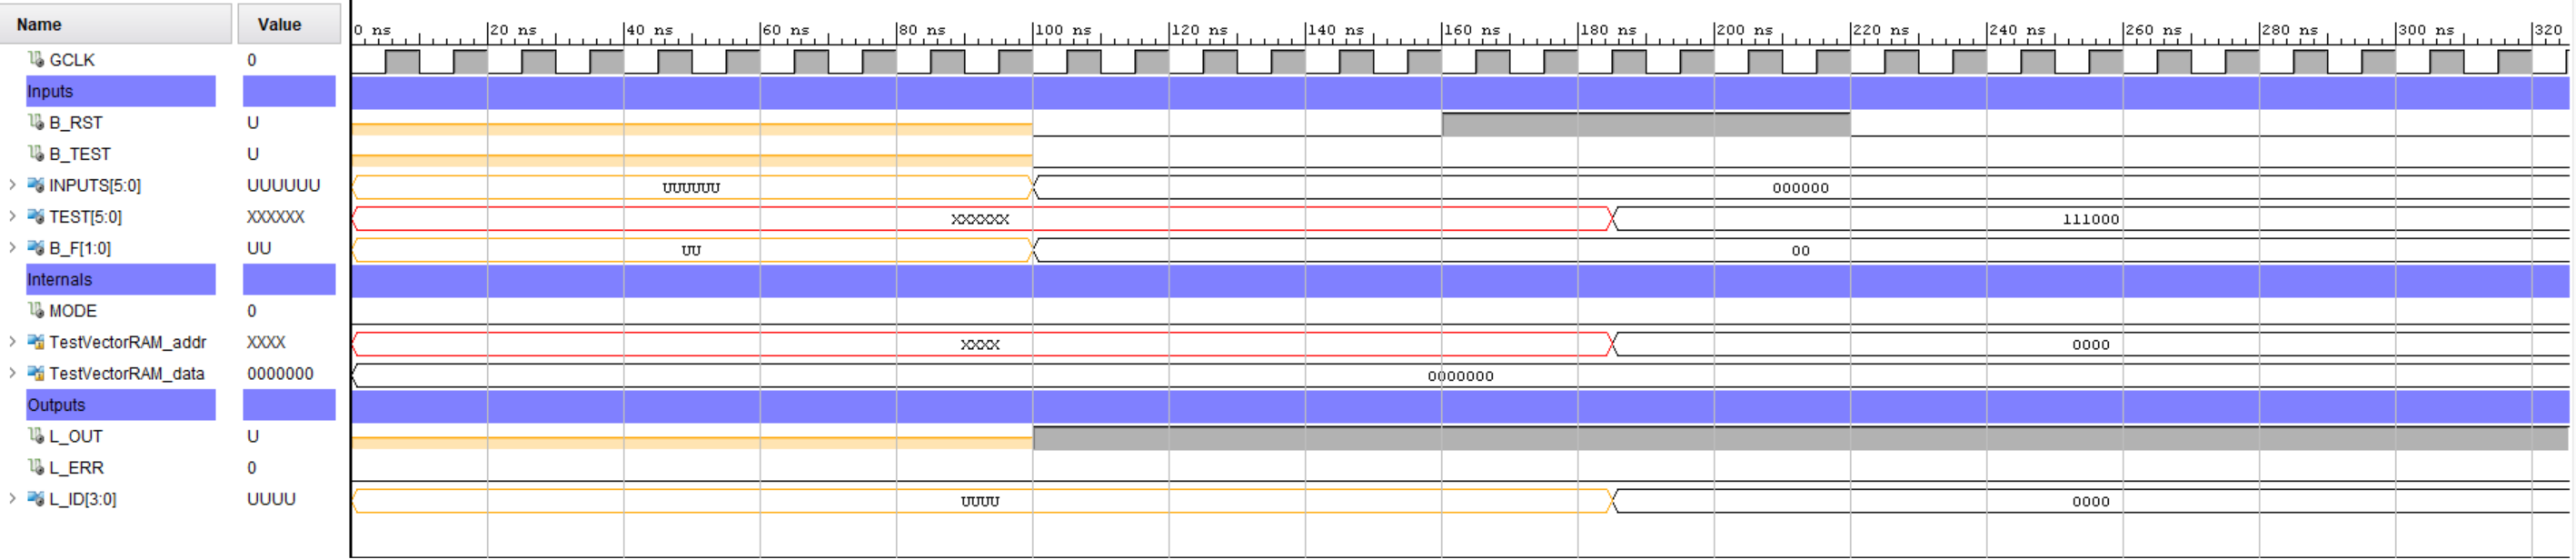
\includegraphics[width=\columnwidth]{Assets/3.2.3_reset.png}
\end{figure}

\subsection*{Waveform 2: Test 1}
\begin{figure}[H]
    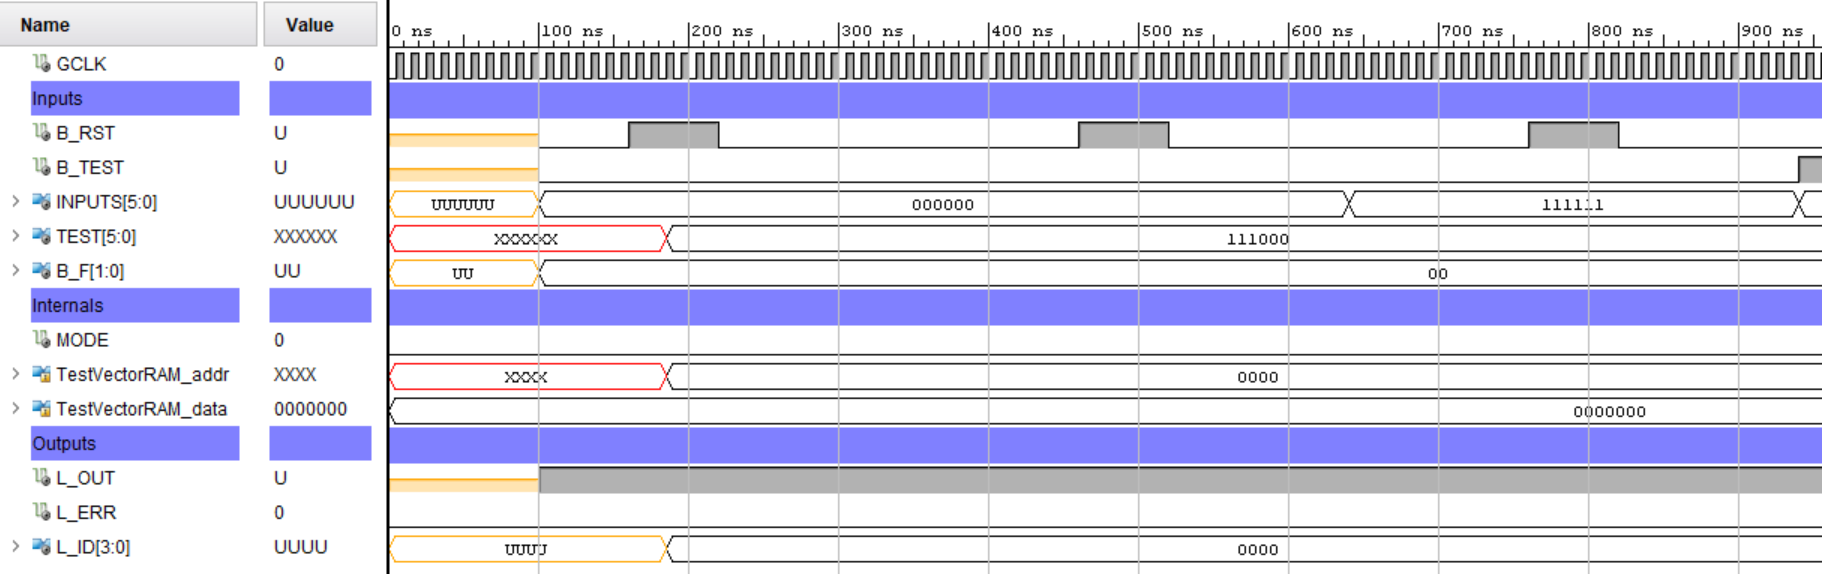
\includegraphics[width=\columnwidth]{Assets/3.2.3_test1.png}
\end{figure}

\subsection*{Waveform 3: Test 2}
\begin{figure}[H]
    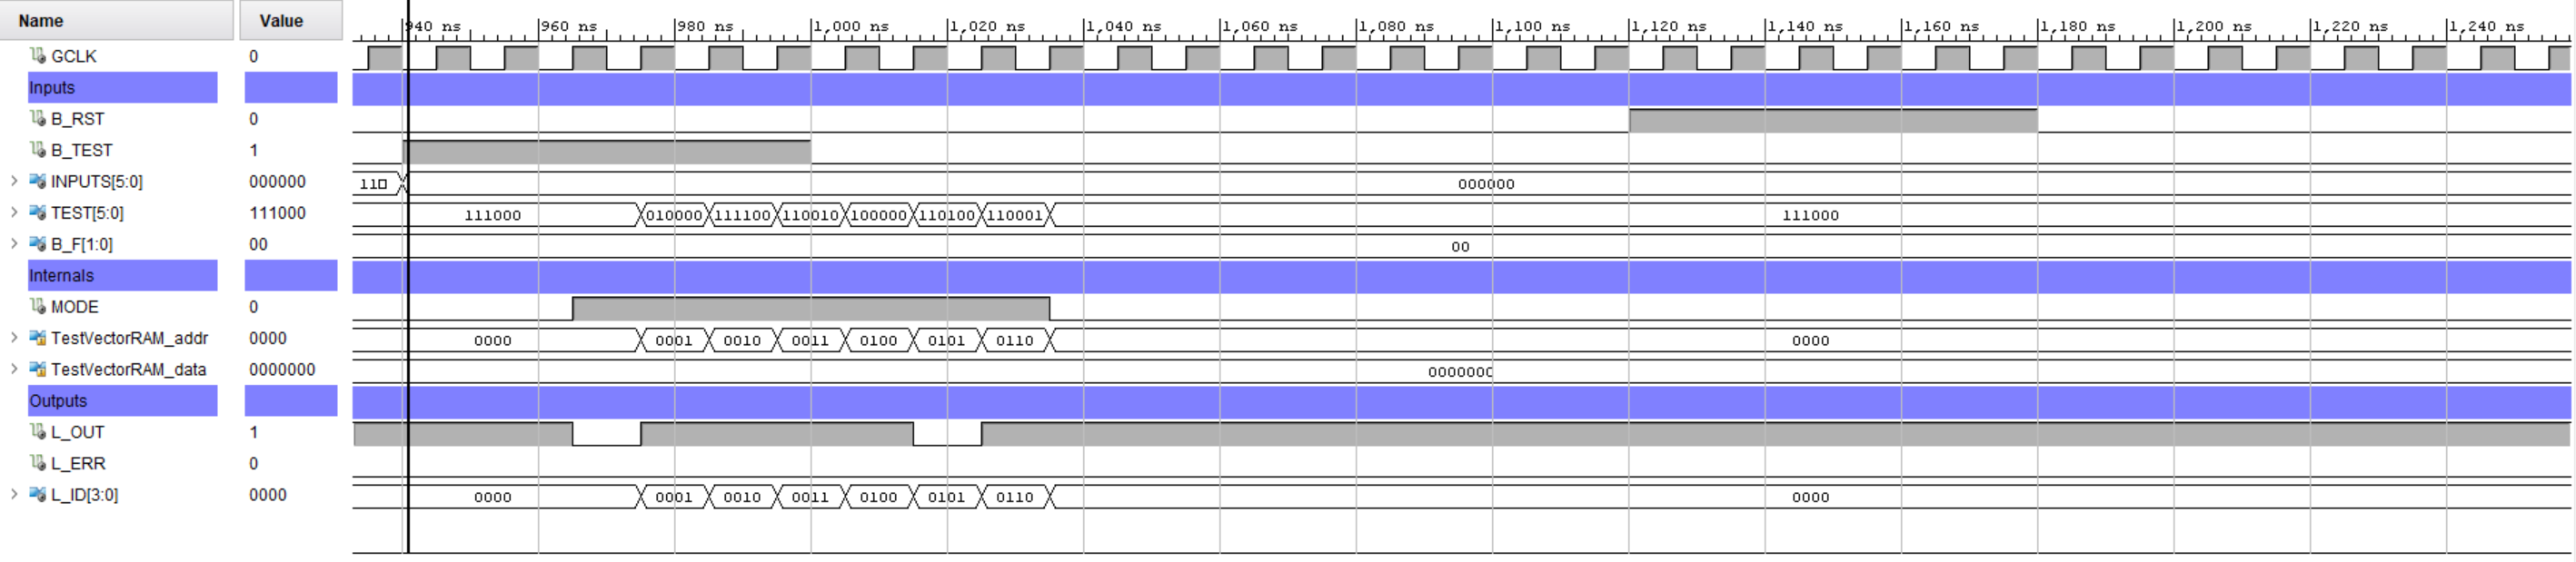
\includegraphics[width=\columnwidth]{Assets/3.2.3_test2.png}
\end{figure}

\subsection*{Waveform 4: Test 3}
\begin{figure}[H]
    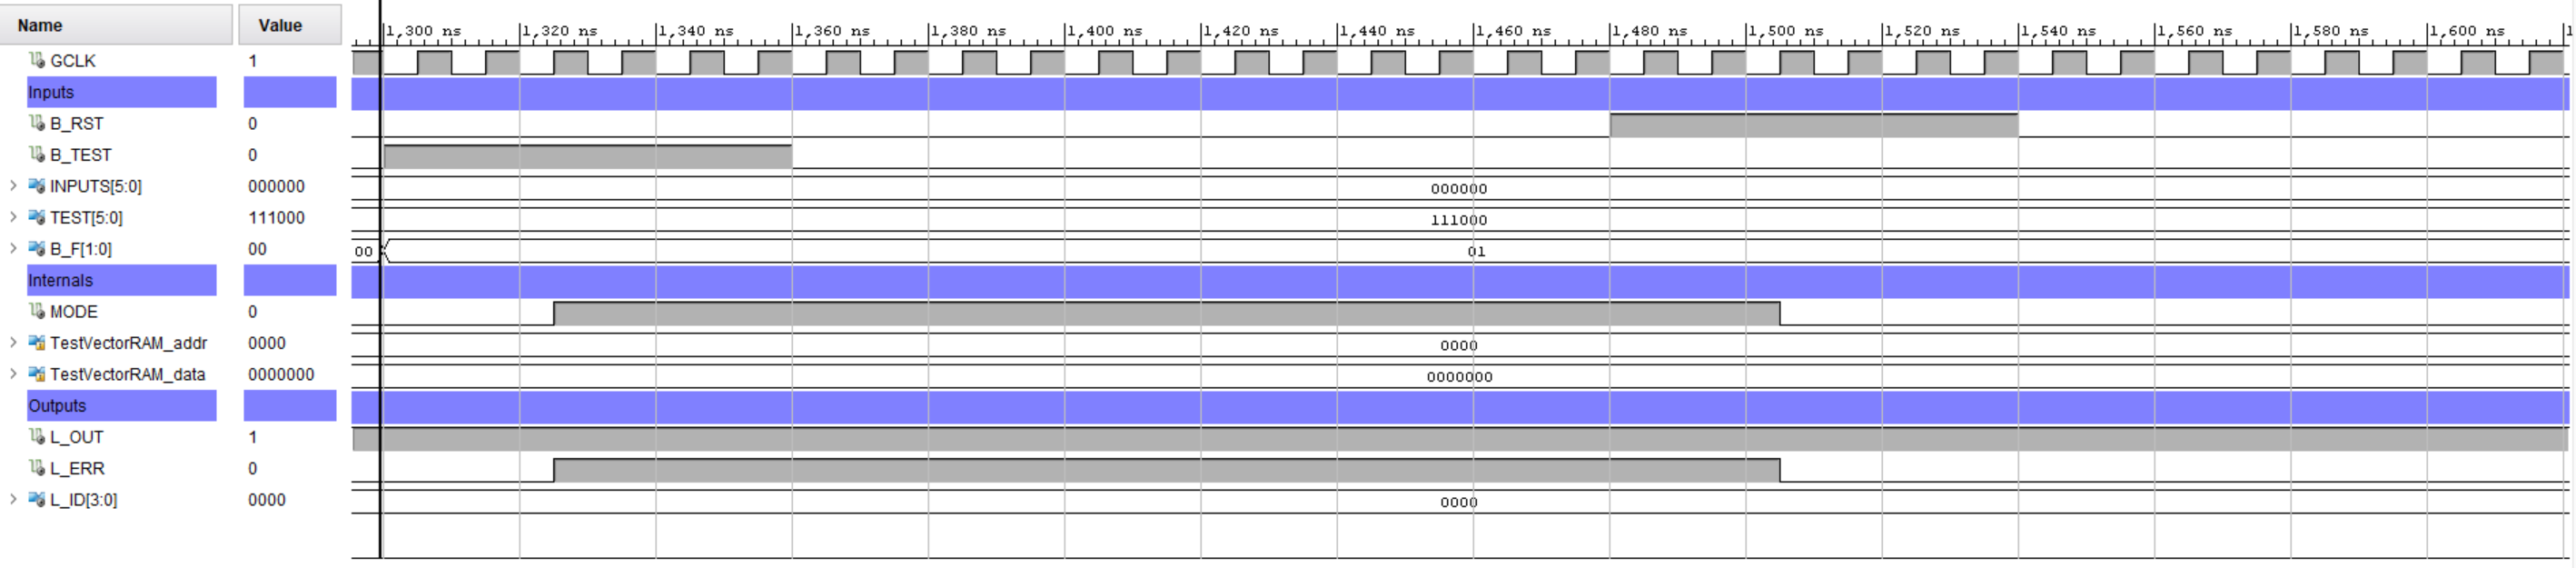
\includegraphics[width=\columnwidth]{Assets/3.2.3_test3.png}
\end{figure}

We can see `L\_ERR' turning high as the Es-a-1 fault is detected by the first test vector in memory, the one that detects the Ds-a-1 fault (111000). This verifies that the tests are correct as the table in section 3.1.6 shows Ds-a-1 can verify Es-a-1.


\subsection*{Waveform 5: Test 4}
\begin{figure}[H]
    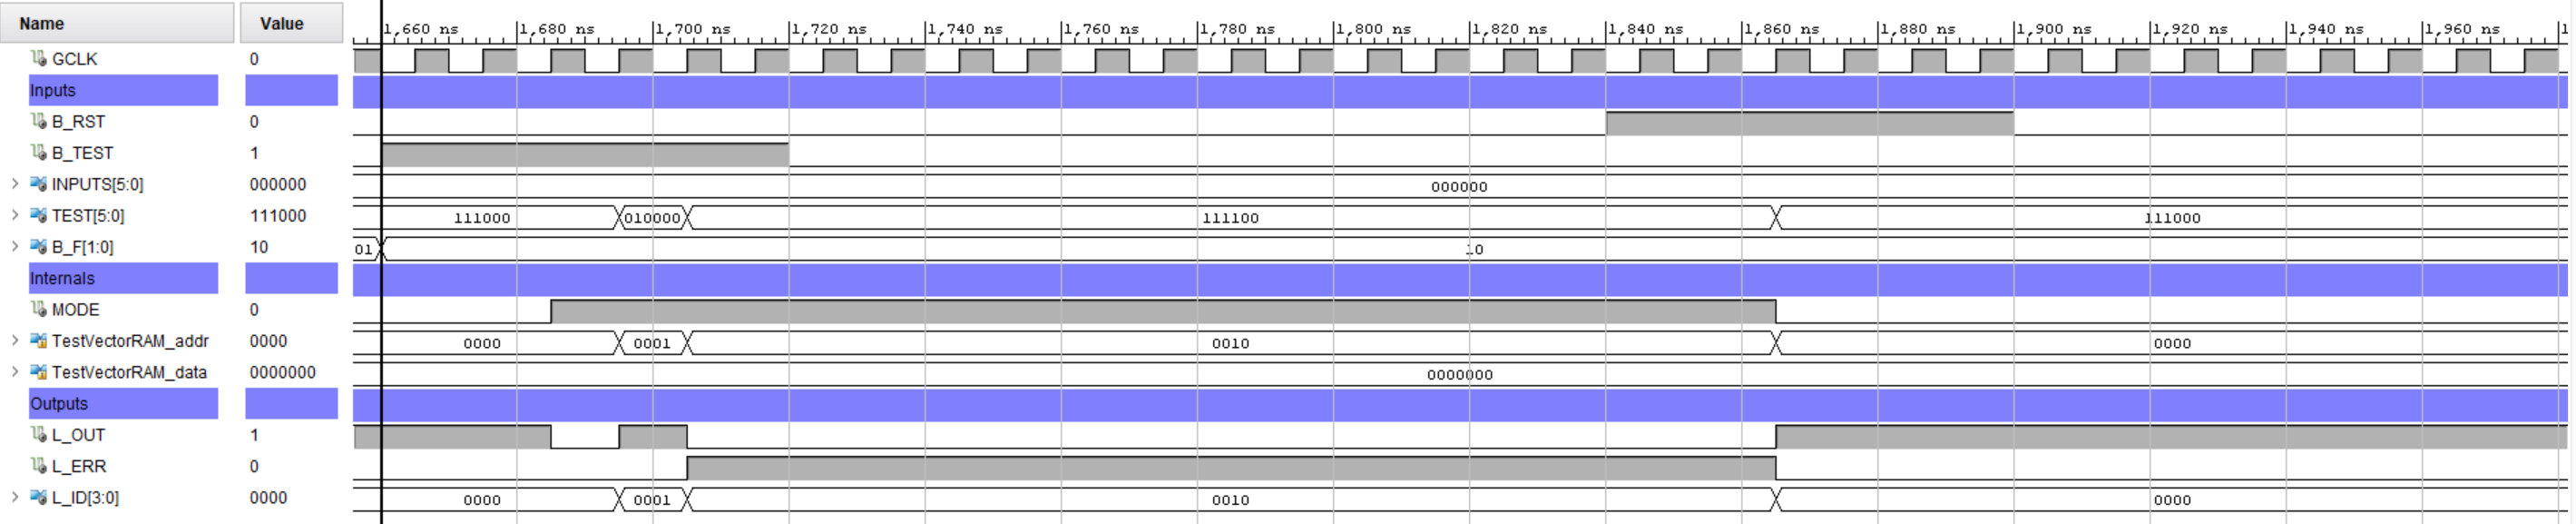
\includegraphics[width=\columnwidth]{Assets/3.2.3_test4.png}
\end{figure}

Here we can see `L\_ERR' going high as the Hs-a-0 fault is detected by the third test vector in memory, the one that detects the Cs-a-0 fault (111100). Again, this verifies that the tests are correct as the table in section 3.1.6 shows Cs-a-0 can verify the Hs-a-0 fault.


\subsection*{Waveform 5: Test 5}
\begin{figure}[H]
    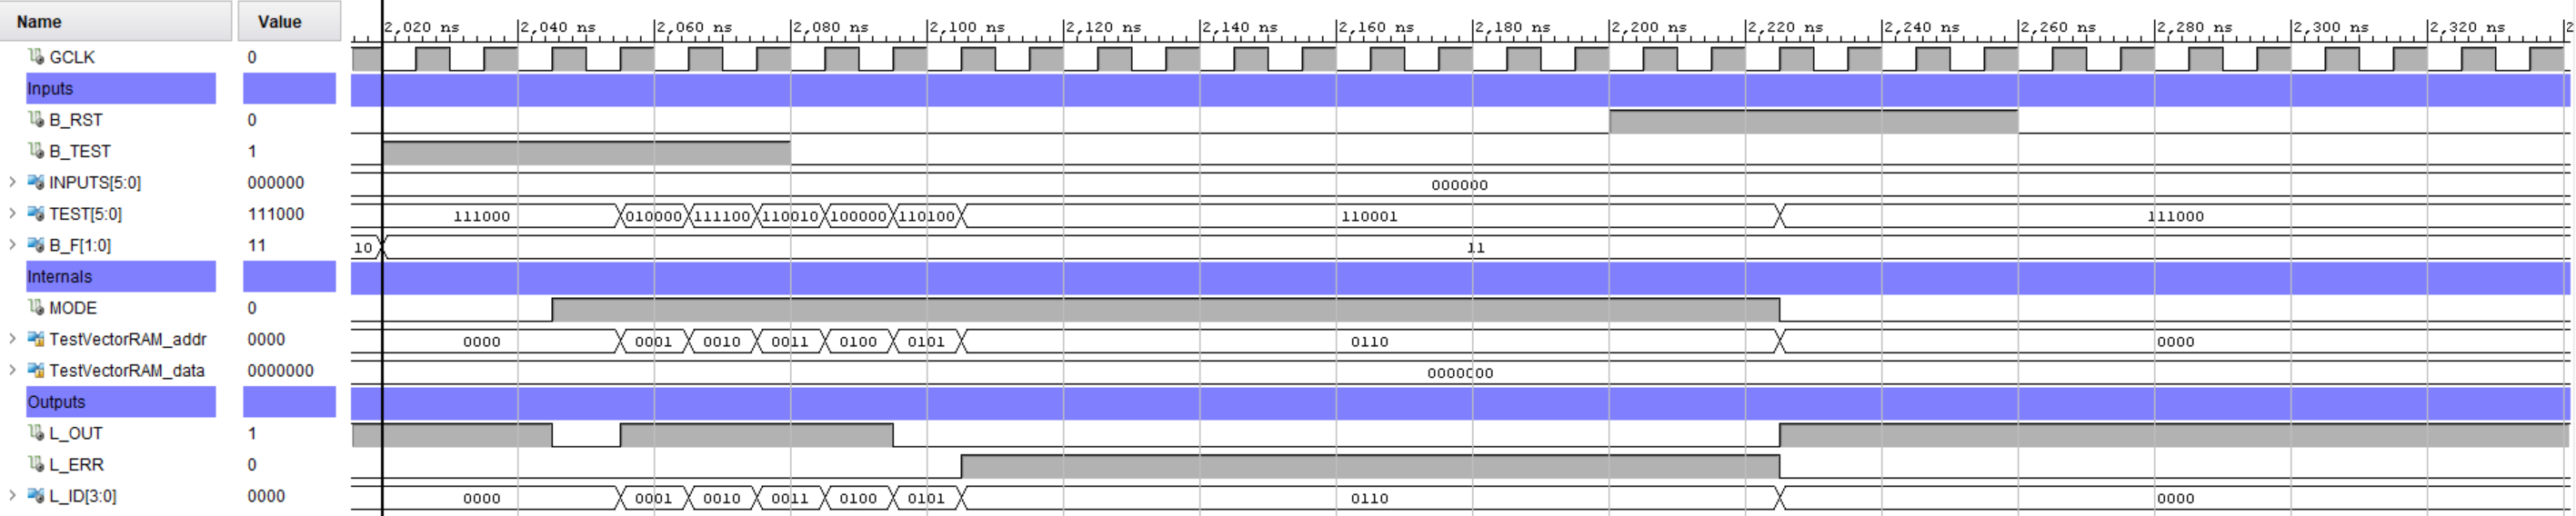
\includegraphics[width=\columnwidth]{Assets/3.2.3_test5.png}
\end{figure}

The signal `L\_ERR' goes high as the Fs-a-0 fault is detected by the last test vector in memory, the one that detects the Fs-a-0 fault (110001).


\section*{3.3.1 Phase Shift and Duty Cycle in a Clock Signal}
\begin{figure}[H]
    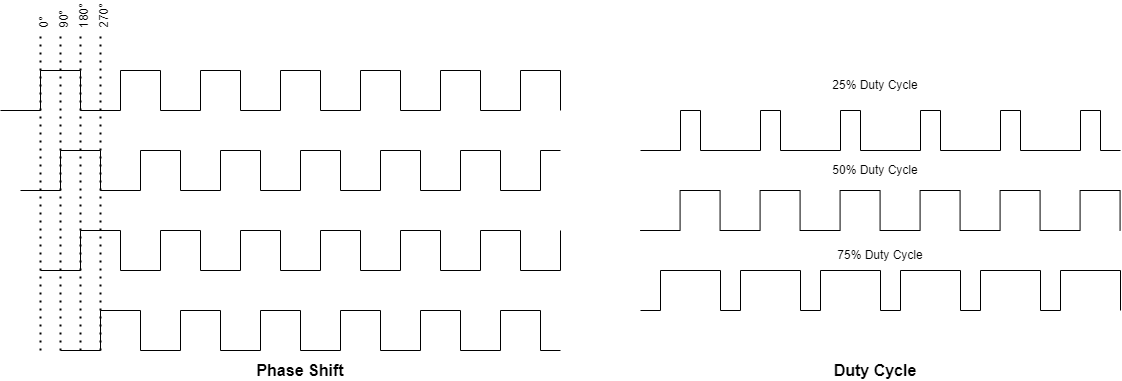
\includegraphics[width=\columnwidth]{Assets/3.3.1_diagrams.png}
\end{figure}

The phase shift of a clock signal refers to the displacement of the signal in time relative to some reference point such as a rising edge. For example, if we have a clock signal with a period of 1 microsecond and a phase shift of 90$^{\circ}$, the clock signal will be shifted by 0.5 microseconds relative to the rising edge reference point. The diagram above shows phase shifts of 0$^{\circ}$, 90$^{\circ}$, 180$^{\circ}$ and 270$^{\circ}$.

The duty cycle of a clock signal is the percentage of time that the signal is in the `high' state. It is the ratio of the time that the signal spends in the `high' state to the total period of the signal. For example, if we have a clock signal with a period of 1 microsecond and a duty cycle of 50\%, the signal will be high for 0.5 microseconds and low for the remaining 0.5 microseconds. The diagram above shows duty cycles of 25\%, 50\% and 75\%.




\section*{3.3.2 Behavioural Simulation}
\subsection*{Waveform 1: Global Reset \& Initialisation}
\begin{figure}[H]
    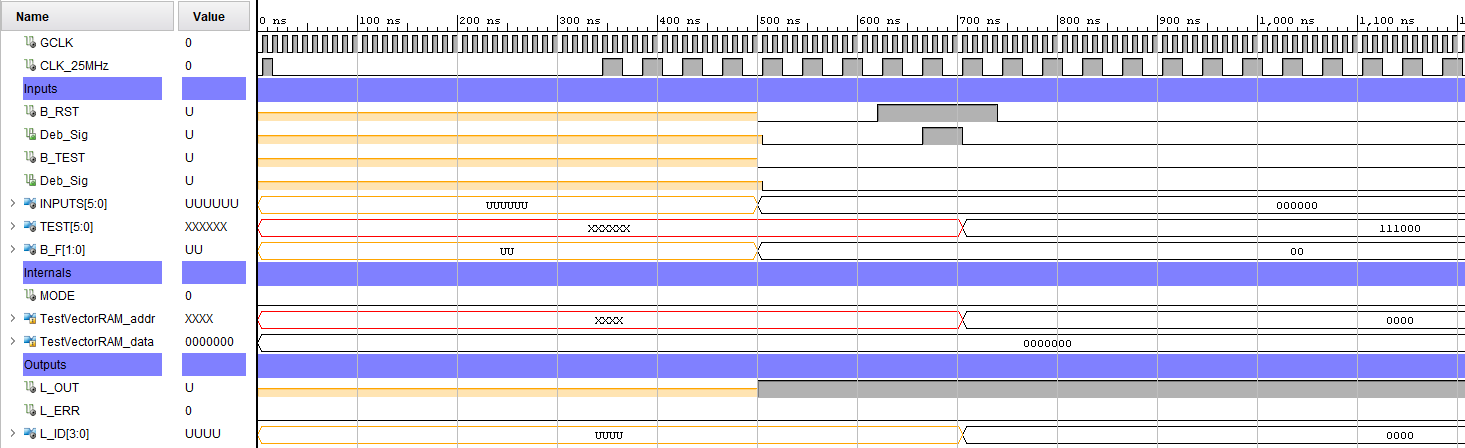
\includegraphics[width=\columnwidth]{Assets/3.3.2_reset.png}
\end{figure}

\subsection*{Waveform 2: Test 1}
\begin{figure}[H]
    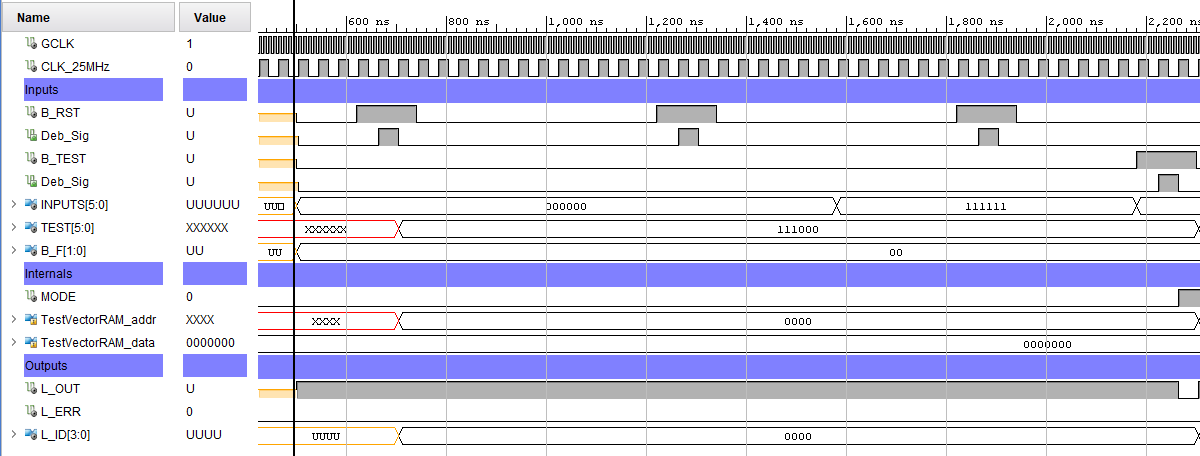
\includegraphics[width=\columnwidth]{Assets/3.3.2_test1.png}
\end{figure}

\subsection*{Waveform 3: Test 2}
\begin{figure}[H]
    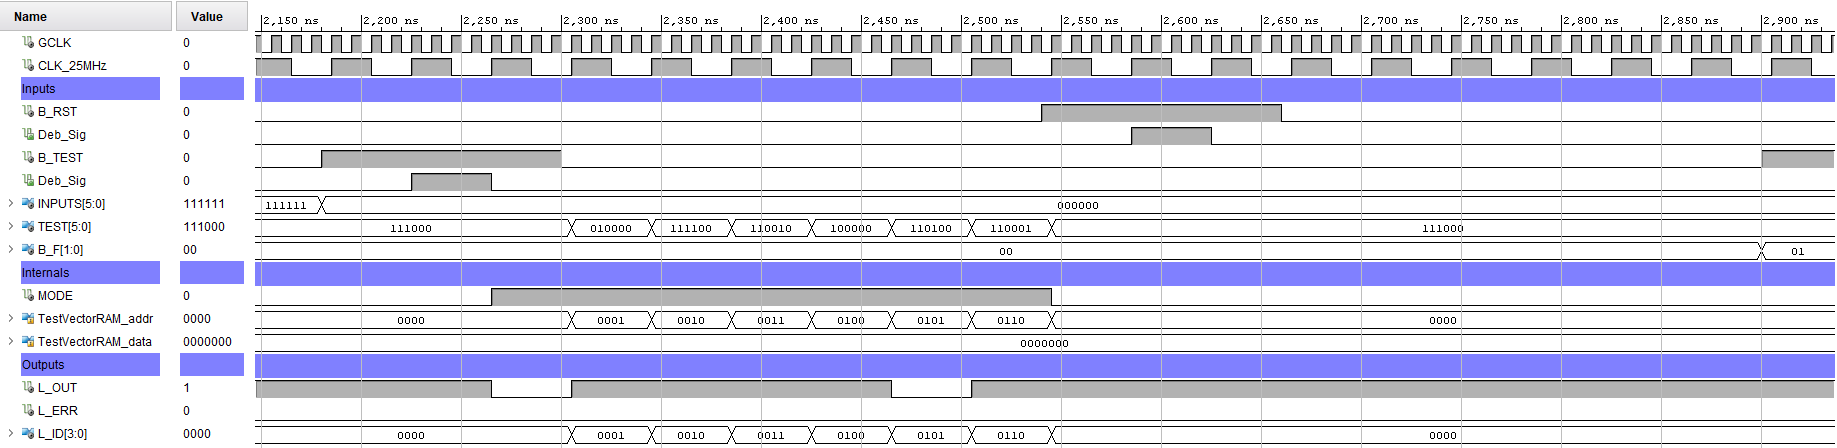
\includegraphics[width=\columnwidth]{Assets/3.3.2_test2.png}
\end{figure}

\subsection*{Waveform 4: Test 3}
\begin{figure}[H]
    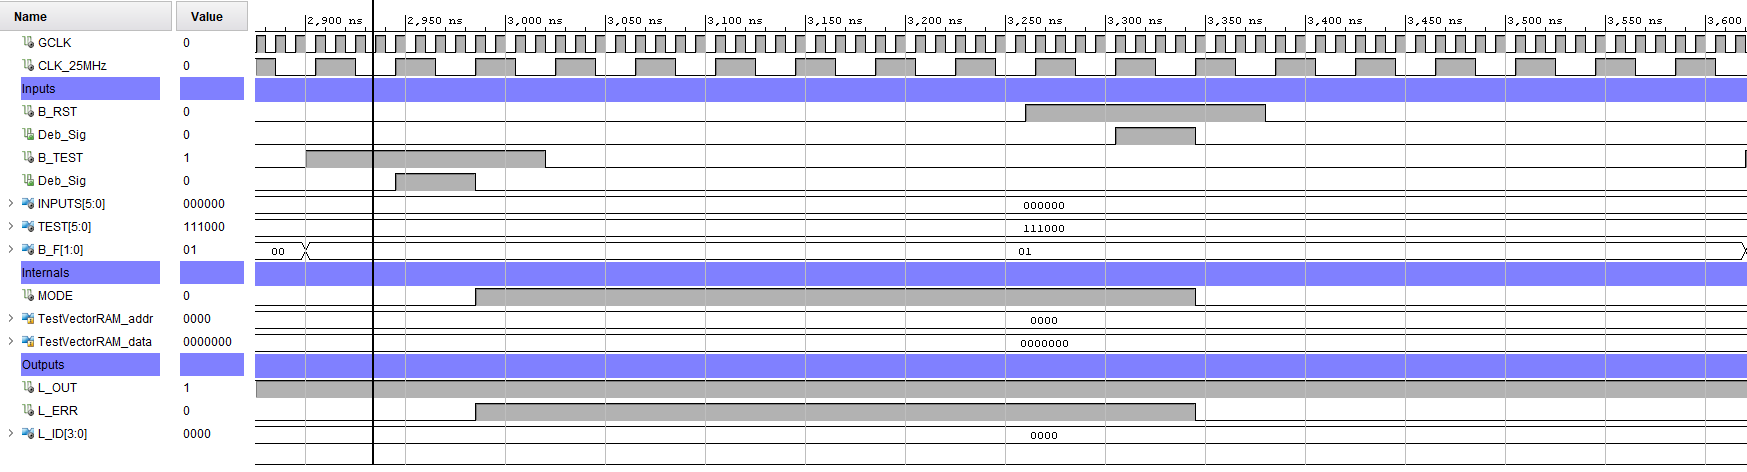
\includegraphics[width=\columnwidth]{Assets/3.3.2_test3.png}
\end{figure}

\subsection*{Waveform 5: Test 4}
\begin{figure}[H]
    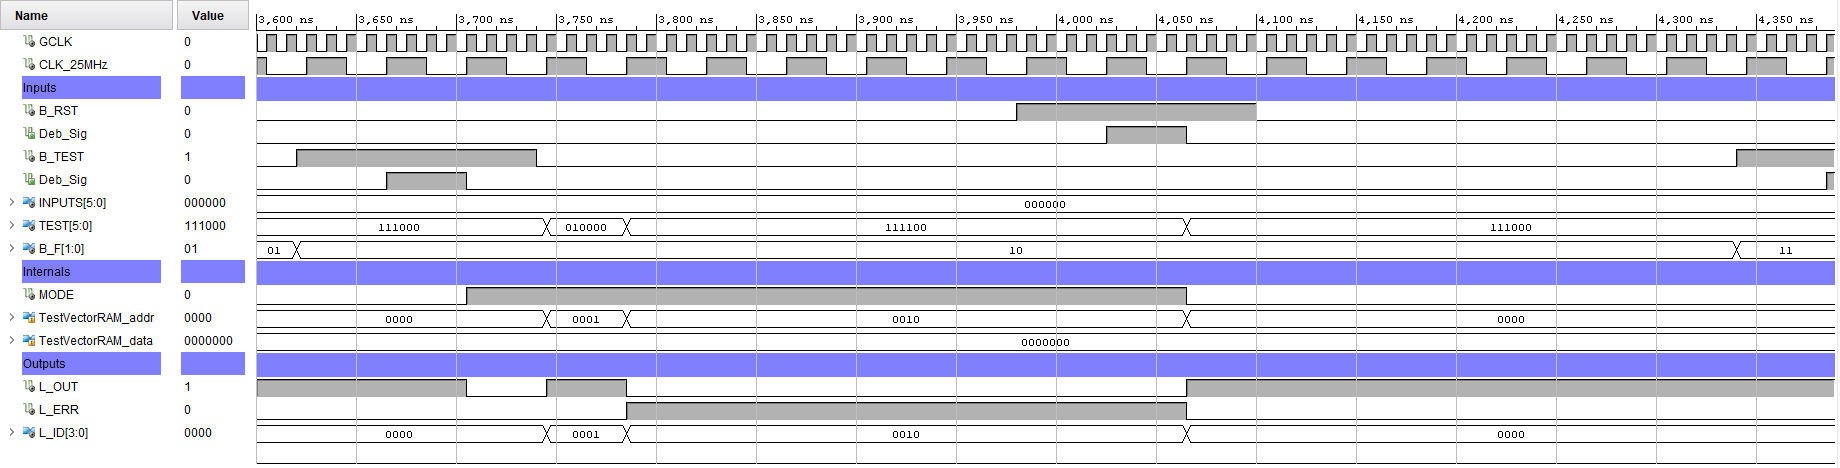
\includegraphics[width=\columnwidth]{Assets/3.3.2_test4.png}
\end{figure}

\subsection*{Waveform 5: Test 5}
\begin{figure}[H]
    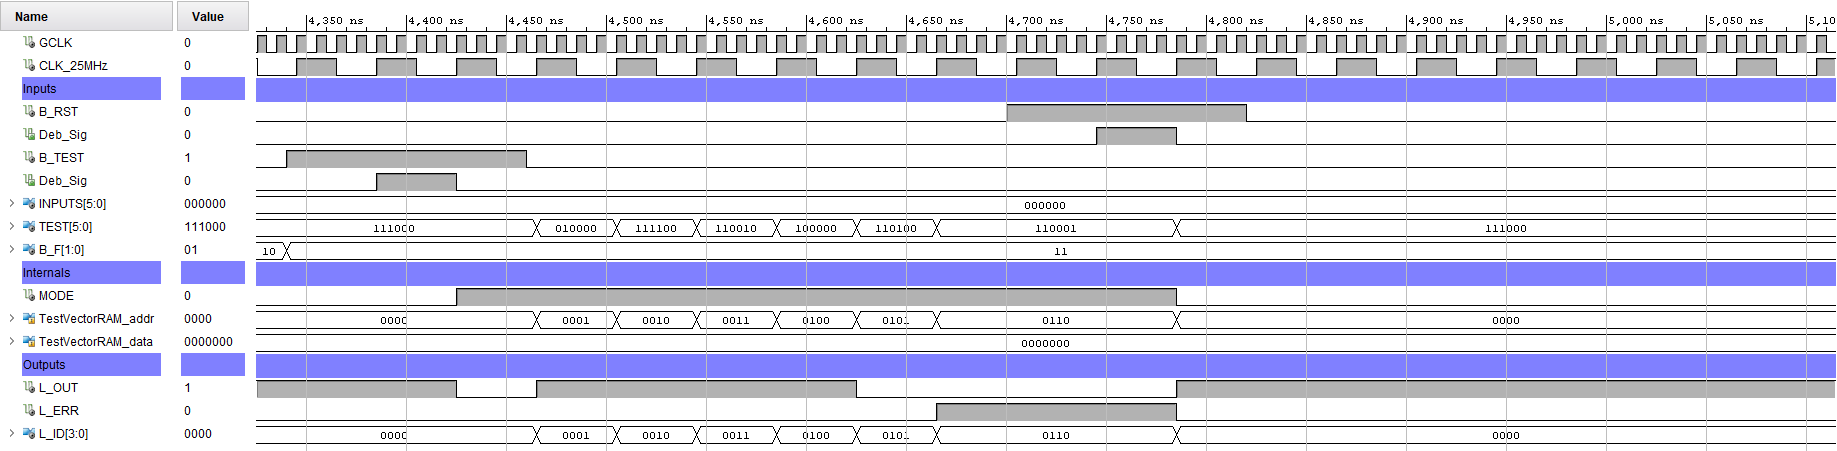
\includegraphics[width=\columnwidth]{Assets/3.3.2_test5.png}
\end{figure}


\section*{3.3.3 ILA Simulation}
\subsection*{Waveform 1: Fault Free Cycle}
\begin{figure}[H]
    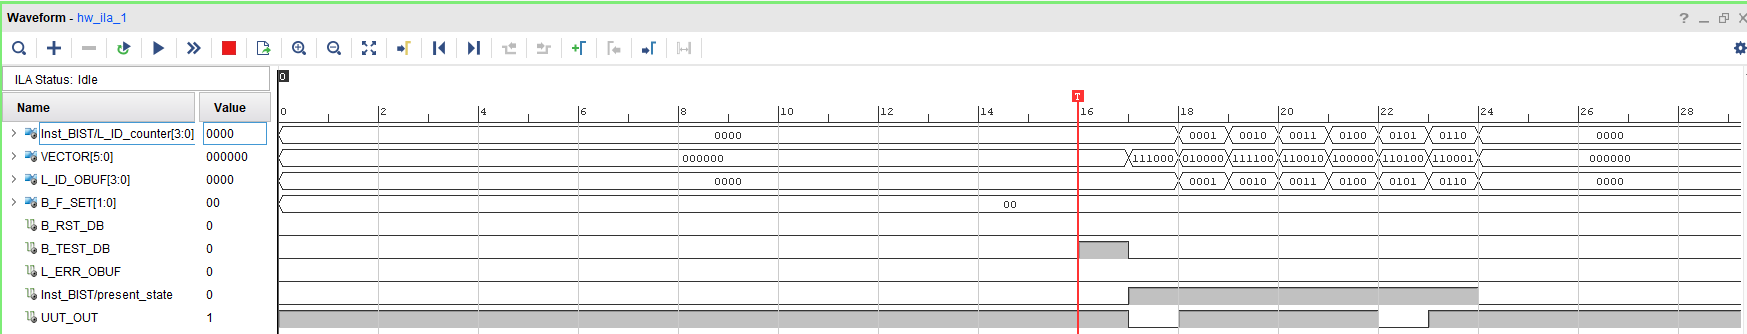
\includegraphics[width=\columnwidth]{Assets/3.3.3_fault-free.png}
\end{figure}

\subsection*{Waveform 2: Es-a-1 Fault}
\begin{figure}[H]
    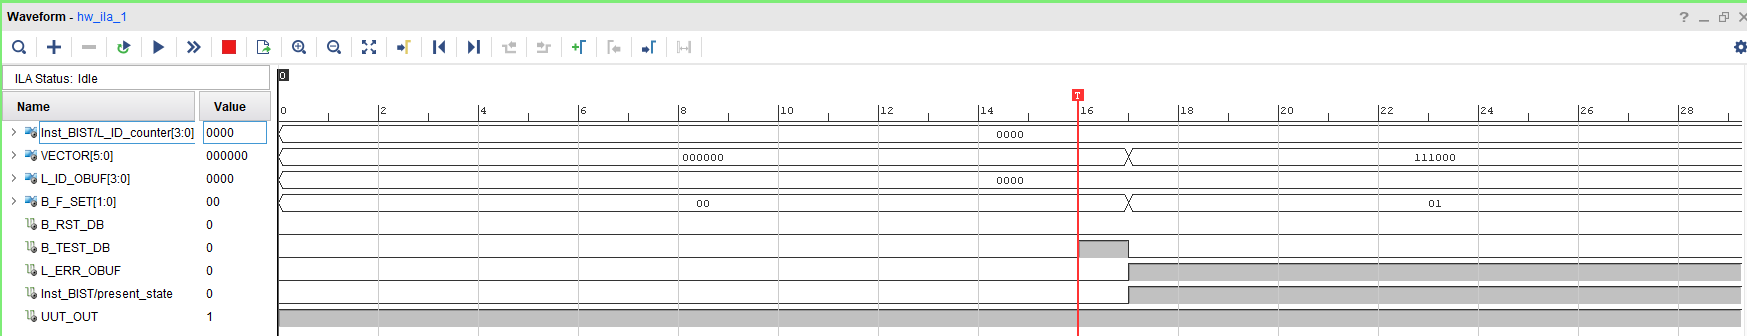
\includegraphics[width=\columnwidth]{Assets/3.3.3_fault-1.png}
\end{figure}

\subsection*{Waveform 3: Hs-a-0 Fault}
\begin{figure}[H]
    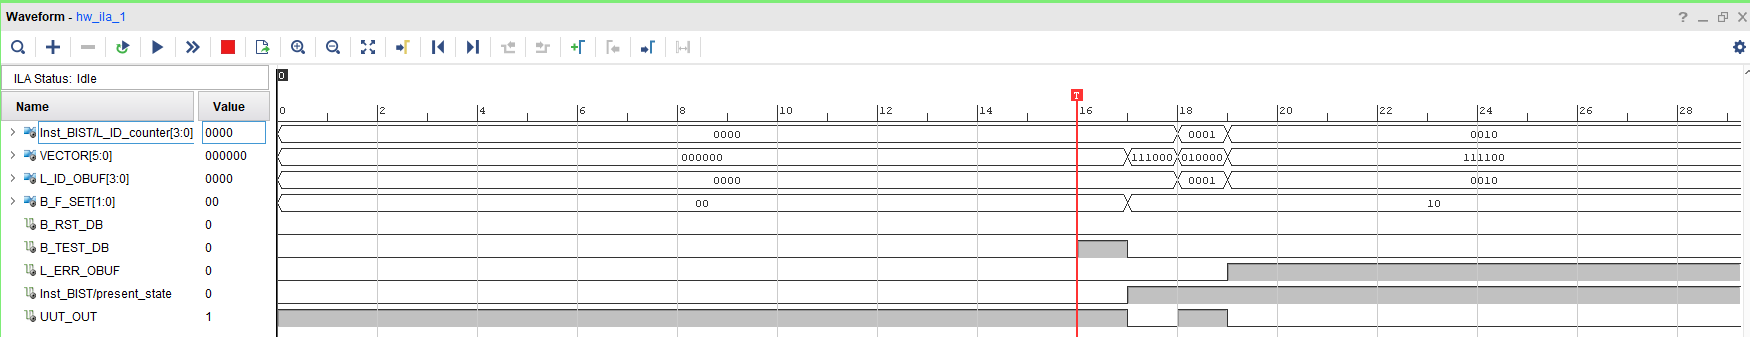
\includegraphics[width=\columnwidth]{Assets/3.3.3_fault-2.png}
\end{figure}

\subsection*{Waveform 4: Fs-a-0 Fault}
\begin{figure}[H]
    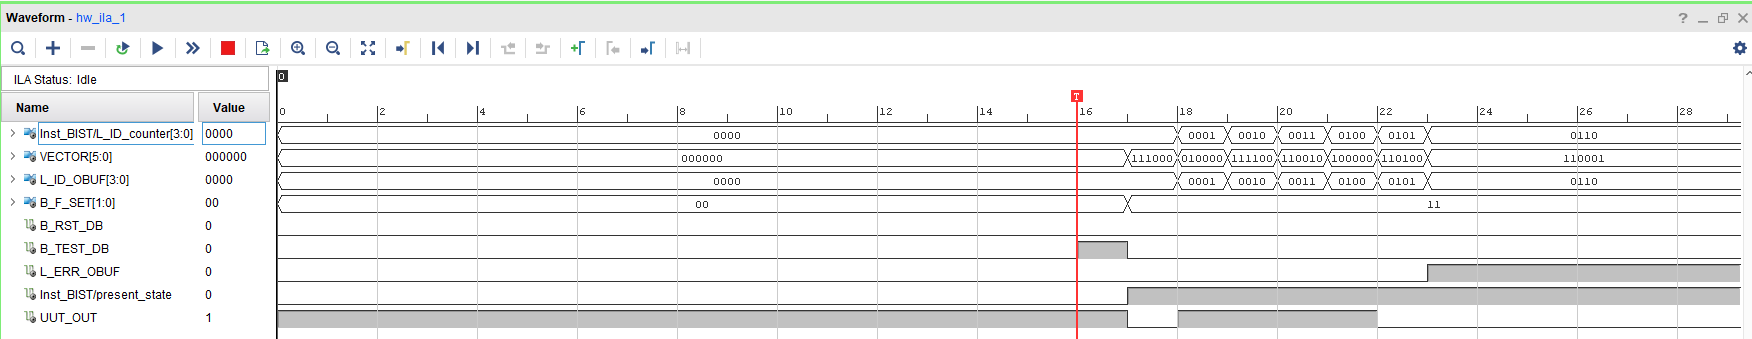
\includegraphics[width=\columnwidth]{Assets/3.3.3_fault-3.png}
\end{figure}

\section*{3.3.4 Nyquist Theorem and the ILA}
The Nyquist theorem states that a signal must be sampled with a rate of at least twice the highest frequency of the signal. However, with an internal logic analyser (ILA), digital signals are sampled instead of analogue ones.

Digital signals are represented by discrete `high’ and `low’ voltage states, therefore, the required sampling rate is not dependent on the highest frequency of the signal, but instead is dependent on the rate of level change of the signals.

\end{document}
